%---------------------------------------------------------------------------------------------------
%		thesis.tex
%
%	This is the master file of the LaTeX document and contains all the directives that compilers use
% to build the document.
%
%	Author: Andrea Meneghinello
% Version: 0.1
%	Table of changes:
%		15/03/2016 -> document definition
%---------------------------------------------------------------------------------------------------
%---------------------------------------------------------------------------------------------------
%    Preamble.tex
%
%	This file define the preamble for current document and in particular it contains all the include
% directives to import the necessary packages and styles to correctly build the document. It also
% defines user specified macros that help writers to write the document.
%
% Author: Andrea Meneghinello
% Version: 0.1
% Table of changes:
%		15/03/2016 -> document definition
%---------------------------------------------------------------------------------------------------
\documentclass[paper=A4, fontsize=11pt, openright, parskip=full, twoside]{scrreprt}

\usepackage{acronym}
\usepackage{abstract}
\usepackage{caption}
\usepackage{etoolbox}
\usepackage{graphicx}
\usepackage{ifthen}
\usepackage{lastpage}
\usepackage{lipsum}
\usepackage{longtable}
\usepackage{multirow}
\usepackage{nameref}
\usepackage{pdfpages}
\usepackage{sectsty}
\usepackage{siunitx}
\usepackage{subcaption}
\usepackage[page, toc]{appendix}
\usepackage[english]{babel}
\usepackage[style=numeric, useprefix, hyperref, backend=bibtex]{biblatex}
\usepackage[utf8]{inputenc}
\usepackage[babel]{csquotes}
\usepackage[T1]{fontenc}
\usepackage[hidelinks]{hyperref}
\usepackage[nonumberlist, toc]{glossaries}
\usepackage[expansion=true, protrusion=true]{microtype}
\usepackage[automark, headsepline, markuppercase]{scrpage2}

%
%	Command to retrieve the current section
%
\makeatletter{}
\newcommand*{\current}{\@currentlabelname}

\def\thischaptertitle{}
\apptocmd{\@chapter}{\gdef\thischaptertitle{#1}}{}{}

\newcommand{\DeclareDividedList}[1]%
{\newcounter{#1@chapter}\setcounter{#1@chapter}{0}}

\pretocmd{\addcontentsline}%
{\ifltxcounter{#1@chapter}%
	{%
		\ifnumgreater{\thechapter}{\value{#1@chapter}}{%
			\setcounter{#1@chapter}{\thechapter}%
			\addtocontents{#1}{\protect\contentsline{chapter}%
				{\protect\numberline {\thechapter} {\thischaptertitle}}{}{} }
		}{}%
	}{}%
}{}{}

\makeatother{}

\DeclareDividedList{lof}
\DeclareDividedList{lot}

%
%	Set title page style
%
\allsectionsfont{\centering{ \normalfont{\scshape{}}}}

%
%	Header and footer page style
%
\pagestyle{scrheadings}
\clearscrheadfoot{}
\lehead{MSc in Computer Science}
\chead{}
\rohead{\current}
\cfoot{\thepage{} of \pageref{LastPage}}

%
% Glossary style
%
\setglossarystyle{altlist}
\makeglossaries{}

%
% Constant definition
%
\newcommand{\FALSE}{false}
\newcommand{\TRUE}{true}

%
% Macro definition
%
\newcommand{\glossaryPlr}[1]{\underline{\glspl{#1}}}
\newcommand{\glossarySng}[1]{\underline{\gls{#1}}}
\newcommand{\keyword}[1]{\textbf{#1}}
\newcommand{\printLOF}[1]{\ifthenelse{\equal{#1}{\TRUE{}}}{\listoffigures{}}{}}
\newcommand{\printLOT}[1]{\ifthenelse{\equal{#1}{\TRUE{}}}{\listoftables{}}{}}
\newcommand{\printTOC}[1]{\ifthenelse{\equal{#1}{\TRUE{}}}{\tableofcontents{}}{}}
\newcommand{\printGLS}[1]{\ifthenelse{\equal{#1}{\TRUE{}}}{\clearpage{}\printglossary[title=Glossary]{}}{}}

%
% Command re-definition
%
%\renewcommand{\thefigure}{\arabic{figure}}
\renewcommand{\thetable}{\arabic{table}}
\renewcommand{\appendixname}{Appendices}
\renewcommand\appendixpagename{\usekomafont{disposition}Appendices}

%
%	Link to database file
%
%---------------------------------------------------------------------------------------------------
%	acronym.tex
%
% This is the acronym database file. Users must write here the acronym definitions before using them
% in the document.
%
% Author:  Andrea Meneghinello
% Version: 0.1
% Table of changes:
%		15/03/2016 -> document definition
%---------------------------------------------------------------------------------------------------
\acrodef{abi}[ABI]{Application Binary Interface}
\acrodef{am}[AM]{Availability Management}
\acrodef{api}[API]{Application Programming Interface}
\acrodef{amqp}[AMQP]{Advanced Message Queuing Protocol}
\acrodef{aws}[AWS]{Amazon Web Services}

\acrodef{bios}[BIOS]{Basic Input/Output System}
\acrodef{blas}[BLAS]{Basic Linear Algebra Subroutine}
\acrodef{bsd}[BSD]{erkeley Software Distribution}

\acrodef{caa}[CaA]{Cloud as Architecture}
\acrodef{caas}[CaaS]{Container as a Service}
\acrodef{capex}[CAPEX]{CAPtial EXpenditures}
\acrodef{ceo}[CEO]{Chief Execution Officier}
\acrodef{cicd}[CI/CD]{Continous Integration/Continous Delivery}
\acrodef{cli}[CLI]{Command Line Interface}
\acrodef{cm}[CM]{Capacity Management}
\acrodef{com}[COM]{Component Object Model}
\acrodef{corba}[CORBA]{Common Object Request Broker Architecture}
\acrodef{cpu}[CPU]{Central Processing Unit}
\acrodef{crm}[CRM]{Content Relationship Management}
\acrodef{csrf}[CSRF]{Cross Site Request Forgery}

\acrodef{dbms}[DBMS]{DataBase Management System}
\acrodef{dfs}[DFS]{Distributed File System}
\acrodef{dos}[DoS]{Denial of Service}
\acrodef{dvd}[DVD]{Digital Verstatile Disk}

\acrodef{ec2}[EC2]{Elastic Cloud Compute}

\acrodef{flops}[FLOPS]{Floating-Point Operations Per Second}
\acrodef{fs}[FS]{File System}

\acrodef{gae}[GAE]{Google App Engine}
\acrodef{gflops}[GFLOPS]{Giga Floating-Point Operations Per Seconds}
\acrodef{gui}[GUI]{Graphic User Interface}

\acrodef{hpc}[HPC]{High Performance Computing}
\acrodef{hpl}[HPL]{High Performance Linpack}
\acrodef{http}[HTTP]{HyperText Transfer Protocol}

\acrodef{iaas}[IaaS]{Infrastructure as a Service}
\acrodef{ict}[ICT]{Information Communication Technology}
\acrodef{ide}[IDE]{Integrated Development Environment}
\acrodef{io}[I/O]{Input/Output}
\acrodef{ip}[IP]{Internet Protocol}
\acrodef{ipc}[IPC]{Inter-Process Communication}
\acrodef{isa}[ISA]{Instruction Set Architecture}
\acrodef{it}[IT]{Information Technology}
\acrodef{itil}[ITIL]{Information Technology Infrastructure Library}

\acrodef{kvm}[KVM]{Kernel-based Virtual Machine}

\acrodef{lamp}[LAMP]{Linux Apache MySql Php}
\acrodef{lan}[LAN]{Local Area Network}
\acrodef{lxc}[LXC]{LinuX Containers}

\acrodef{mau}[MAU]{Monthly Active Users}

\acrodef{nat}[NAT]{Network Address Translation}
\acrodef{nic}[NIC]{Network Interface Card}
\acrodef{nist}[NIST]{National Institute for Standards and Technologies}
\acrodef{nosql}[NoSQL]{Not Structured Query Language}

\acrodef{os}[OS]{Operating System}

\acrodef{opex}[OPEX]{OPerational EXpenditures}

\acrodef{paas}[PaaS]{Platform as a Service}
\acrodef{pci}[PCI]{Peripheral Component Interconnect}

\acrodef{qemu}[QEMU]{Quick EMUlator}
\acrodef{qobiz}[QoBiz]{Quality of Business}
\acrodef{qos}[QoS]{Quality of Service}

\acrodef{ram}[RAM]{Random Access Memeory}
\acrodef{rest}[REST]{REpresentational State Transfer}

\acrodef{saas}[SaaS]{Software as a Service}
\acrodef{sda}[SDA]{Service Design Area}
\acrodef{sdk}[SDK]{Software Development Kit}
\acrodef{sla}[SLA]{Service Level Agreement}
\acrodef{slo}[SLO]{Service Level Objectivess}
\acrodef{soa}[SOA]{Service Oriented Architecture}
\acrodef{sp}[SP]{Service Provider}
\acrodef{spi}[SPI]{SaaS - PaaS - IaaS}
\acrodef{sql}[SQL]{Structured Query Language}
\acrodef{ssd}[SSD]{Solid-State Drive}
\acrodef{sut}[SUT]{System Under Test}

\acrodef{tcp}[TCP]{Transmission Control Protocol}
\acrodef{tlb}[TLB]{Translation Lookaside Buffer}

\acrodef{udp}[UDP]{User Datagram Protocol}
\acrodef{ufs}[UFS]{Union File System}
\acrodef{ui}[UI]{User Interface}
\acrodef{us}[U.S.]{United States}

\acrodef{vfs}[VFS]{Virtual File System}
\acrodef{vm}[VM]{Virtual Machine}
\acrodef{vod}[VOD]{Video On-Demand}
\acrodef{vpn}[VPN]{Virtual Private Network}
%---------------------------------------------------------------------------------------------------
%	glossary.tex
%
% This is the glossary database file. Users must write here the term definitions before using them
% in the document.
%
% Author:  Andrea Meneghinello
% Version: 0.1
% Table of changes:
%		15/03/2016 -> document definition
%---------------------------------------------------------------------------------------------------
\newglossaryentry{deployment-process}
{
	name = {Deployment process},
	plural = {Deployment processes},
	description = {Software deployment include all the activities that make a software system available
		for use. The general deployment process consists of several interrelated activities with possible
		transitions between them.}
}

\newglossaryentry{bug}
{
	name = {bug},
	plural = {bugs},
	description={A software bug is an error, flaw, failure or fault in a computer program or system that
		 causes it to produce an incorrect or unexpected result, or to behave in unintended ways}
}

\newglossaryentry{pay-per-use}
{
	name = {pay-per-use},
	plural = {pay-per-use},
	description = {Metered services is any type of payment structure in which
		a customer has access to potentially unlimited resources but only pays for what they actually use.
		Metered services are becoming increasingly common in enterprise \acs{it} environments. With utility
		computing, for example, a company can purchase computation resources to  match fluctuating needs.
		This approach is promoted as being more cost-effective for the company than maintaining a large
		infrastructure that exceeds the company's average computing power requirements}
}

\newglossaryentry{cloudInfrastructure}
{
	name = {Cloud Infrastructure},
	plural = {Cloud infrastructures},
	description={A Cloud Infrastructure is the collection of hardware and
		software that enables the five essential characteristics of Cloud Computing. The Cloud Infrastructure
		can be seen as containing both a physical layer and an abstraction layer. The physical layer consists
		of the hardware resources necessary to support the cloud services being provided, and typically
		includes server, storage and network components. The abstraction layer consists of software deployed
		across the physical layer, which manifests the essential Cloud characteristics. Conceptually the
		abstraction layer sits above the physical layer}
}

\newglossaryentry{middleware}
{
	name = {Middleware},
	plural = {Middleware},
	description = {Middleware is a set of software that act as brokers between infrastructures and software,
		allowing communication despite different communication protocols or \acs{os}}
}

\newglossaryentry{agile}
{
	name = {Agile software development},
	description = {agile software development is a group of software development methodologies based on
		incremental development}
}

\newglossaryentry{gartner}
{
	name = {Gartner Magic Quadrant},
	plural = {Gartner Magic Quadrants},
	description = {Gartner Magic Quadrants offer visual snapshots, in-depth analyses and actionable advice
		that provide insight into a market’s direction, maturity and participants. Magic Quadrants compare
		vendors based on Gartner’s standard criteria and methodology. Each report comes with a Magic Quadrant
		graphic that depicts a market using two-dimensional matrix that evaluates vendors based on their
		completeness of vision and ability to execute.}
}
\bibliography{databases/bibliography.bib}

%
%	Add subsub-section to the table of contents
%
\setcounter{tocdepth}{4}
\setcounter{secnumdepth}{4}

\begin{document}
	
	%
	%	Frontispiece of the document
	%
	\includepdf[pages={1}]{frontispiece.pdf}
	\clearpage{}
	
	%
	%	Empty page after the frontispiece inclusion
	%
	\mbox{}
	\thispagestyle{empty}
	\newpage{}
	
	%
	%	Thanks file inclusion
	%
	
	%
	%	Abstract of the document
	%
	\begin{abstract}
		The attention for cloud computing and the take up of its offering have risen swiftly over the last
		decade. The cloud computing stack, also known as \acs{spi}, spans three conceptual layers with
		associated service models: \acs{saas} on the top (at user end), \acs{paas} in the middle (at
		developers end) and finally \acs{iaas} on the bottom (at sysadmin end) where physical resources
		reside.
		
		Owing to more immediate perception of value added, the cloud landscape has shown marked progress
		in the development of the \acs{saas} and \acs{iaas} offerings. Interest in \acs{paas} solutions
		have taken longer to ignite instead, so much so that the \acs{paas} world is still largely unexplored.
		
		The purpose of this thesis is to explore the \acs{paas} layer in order to understand how it is
		different from the \ac{iaas} layer and how we are able to build elastic applications upon it.
		
		We analyse in deep, through the evaluation of infrastructural costs, two units of deployment for
		the \ac{paas} (\acs{vm}s and containerization) in order to choose the better one to host our service.
		Finally, we want to propose a possible software architecture that, through micro-services, is able
		to exploit the elasticity mechanisms provided by the platform.
	\end{abstract}
	
	%
	%	Indexes
	%
	\printTOC{\TRUE{}}
	\printLOT{\TRUE{}}
	\printLOF{\TRUE{}}
	
	%
	% Chapters
	%
	%---------------------------------------------------------------------------------------------------
%		main.tex
%
%	This is the main file of the chapter that talk about elasticity and multi-tenancy.
%
%	Author: Andrea Meneghinello
% Version: 0.1
%	Table of changes:
%		12/03/2016 -> document definition
%---------------------------------------------------------------------------------------------------
\chapter{Elasticity}
\label{cap:solutionSpace}
%TODO -> chapter abstract

%--------------------------------------------------------------------------------------------------
% elasticity.tex
%
% This document define the frontespiece of the presentation
%
% author: Andrea Meneghinello
% version: 0.1
%--------------------------------------------------------------------------------------------------
\section{Elasticity}
\begin{frame}{Elasticity}
	\begin{columns}
		\begin{column}{0.5\textwidth}
			\textbf{elasticity} obtained by
			\begin{itemize}
				\item{\footnotesize{how PaaS exploits IaaS assets}}
				\begin{itemize}
					\item{\scriptsize{computing}}
					\item{\scriptsize{storage}}
					\item{\scriptsize{networking}}
				\end{itemize}
				\item{\footnotesize{how we build our services}}
				\begin{itemize}
					\item{\scriptsize{software architectures}}
					\item{\scriptsize{Software Engineering principles}}
				\end{itemize}
			\end{itemize}
		\end{column}
		\begin{column}{0.5\textwidth}
			\begin{figure}
				\centering{}
				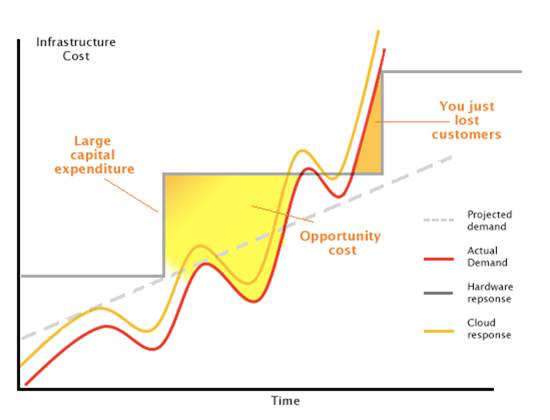
\includegraphics[scale=0.35]{images/elasticity.png}
			\end{figure}
			\begin{flushright}
				\tiny{source: \url{https://goo.gl/EzhyD5}}
			\end{flushright}
		\end{column}
	\end{columns}
\end{frame}

\subsection{Requirements}
\begin{frame}{Requirements}
	\only<1>
	{
		\begin{columns}
			\begin{column}{0.6\textwidth}
				elasticity major requirements
				\begin{itemize}
					\item{\footnotesize{from definition of elasticity}}
					\begin{itemize}
						\item{\scriptsize{autonomy}}
						\item{\scriptsize{scalability $\rightarrow{}$ \textbf{focus on horizontal}}}
						\item{\scriptsize{adaptability}}
					\end{itemize}
					\item{\footnotesize{specific for PaaS layer}}
					\begin{itemize}
						\item{\scriptsize{SLA-awareness}}
						\item{\scriptsize{composability}}
						\item{\scriptsize{service continuity in SW upgrades}}
					\end{itemize}
				\end{itemize}
			\end{column}
			\begin{column}{0.4\textwidth}
				\begin{figure}
					\centering{}
					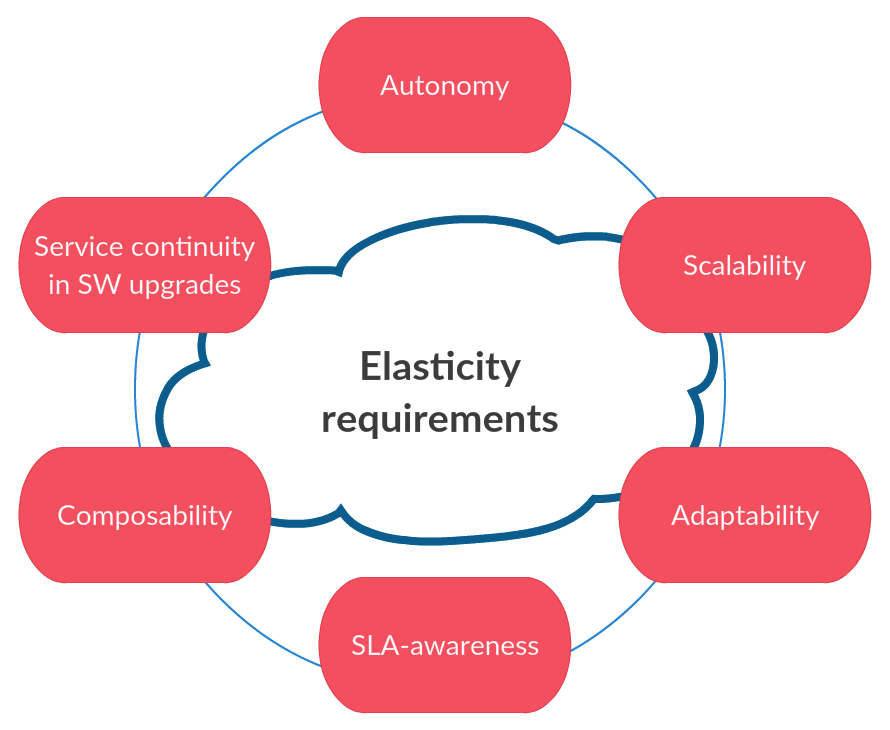
\includegraphics[scale=0.14]{images/elasticity-requirements.png}
				\end{figure}
			\end{column}
		\end{columns}
	}
	\only<2>
	{
		\begin{columns}
			\begin{column}{0.65\textwidth}
				scalability
				\begin{itemize}
					\item{\footnotesize{\textbf{replication (horizontal)}}}
					\begin{itemize}
						\item{\scriptsize{the only possible solution in PaaS}}
						\item{\scriptsize{PaaS manages units of deployments}}
					\end{itemize}
					\item{\footnotesize{some components are replicated when necessary}}
					\begin{itemize}
						\item{\scriptsize{the process must be transparent}}
						\item{\scriptsize{services must be well-designed}}
						\item{\scriptsize{classic architectures does not help}}
					\end{itemize}
					\item{\footnotesize{other}}
					\begin{itemize}
						\item{\scriptsize{redimension (vertical)}}
						\item{\scriptsize{migration}}
					\end{itemize}
				\end{itemize}
			\end{column}
			\begin{column}{0.35\textwidth}
				\begin{figure}
					\centering{}
					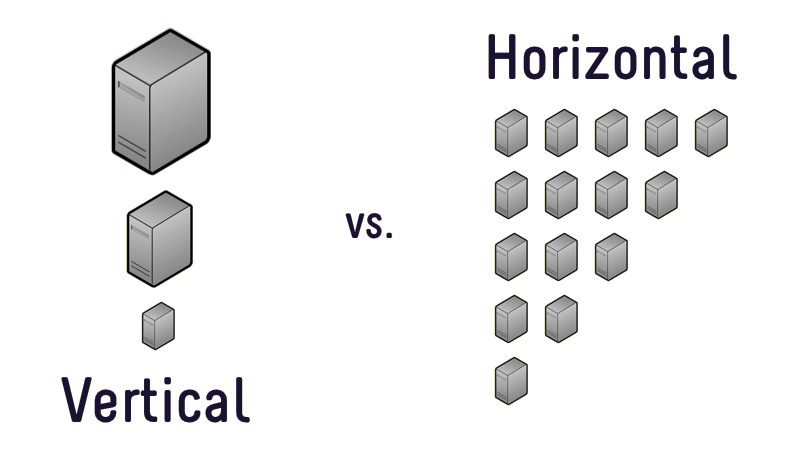
\includegraphics[scale=0.15]{images/scalability.png}
				\end{figure}
				\begin{flushright}
					\tiny{source: \url{https://goo.gl/orFWSi}}
				\end{flushright}
			\end{column}
		\end{columns}
	}
\end{frame}

\subsection{Multi-tenancy}
\begin{frame}{Multi-tenancy}
	\only<1>
	{
		\begin{columns}
			\begin{column}{0.57\textwidth}
				requirements
				\begin{itemize}
					\item{\footnotesize{availability $\rightarrow{}$ redundant services}}
					\item{\footnotesize{secure tenants isolation}}
					\item{\footnotesize{guarantee of service $\rightarrow$ performance}}
					\item{\footnotesize{management of underlying resources}}
				\end{itemize}
				\begin{center}
					providers have to plan SLA with a rich set of \textbf{objectives}
				\end{center}
			\end{column}
			\begin{column}{0.43\textwidth}
				\begin{figure}
					\centering{}
					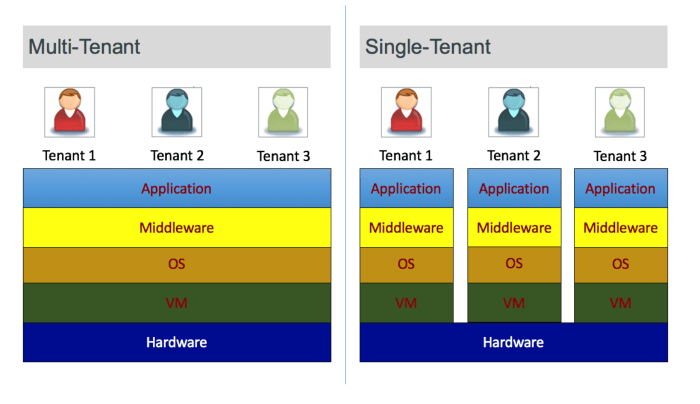
\includegraphics[scale=0.21]{images/multi-tenancy.png}
				\end{figure}
				\begin{flushright}
					\tiny{source: \url{http://goo.gl/MlsmWj}}
				\end{flushright}
			\end{column}
		\end{columns}
	}
	\only<2>
	{
		\begin{columns}
			\begin{column}{0.57\textwidth}
				naive architectures lead to
				\begin{itemize}
					\item{\footnotesize{inflexibility toward different needs}}
					\item{\footnotesize{security lacks}}
					\item{\footnotesize{inadequate usability}}
					\begin{itemize}
						\item{\scriptsize{sustain high workload $\rightarrow{}$ elasticity}}
					\end{itemize}
				\end{itemize}
			\end{column}
			\begin{column}{0.43\textwidth}
				\begin{figure}
					\centering{}
					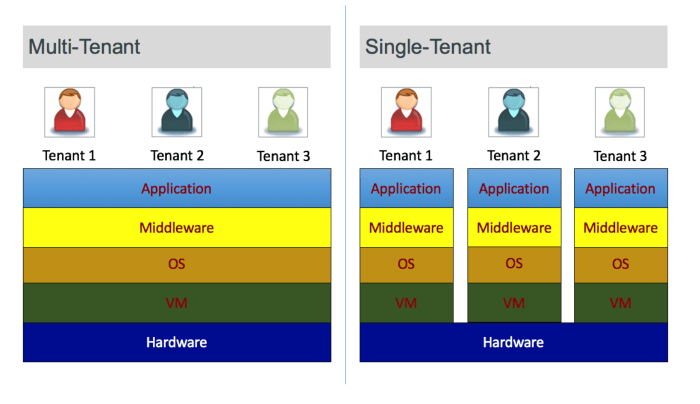
\includegraphics[scale=0.21]{images/multi-tenancy.png}
				\end{figure}
				\begin{flushright}
					\tiny{source: \url{http://goo.gl/MlsmWj}}
				\end{flushright}
			\end{column}
		\end{columns}
	}
\end{frame}
	%---------------------------------------------------------------------------------------------------
%		main.tex
%
%	This is the main file of the chapter that talk about elasticity and multi-tenancy.
%
%	Author: Andrea Meneghinello
% Version: 0.1
%	Table of changes:
%		12/03/2016 -> document definition
%---------------------------------------------------------------------------------------------------
\chapter{Elasticity}
\label{cap:solutionSpace}
%TODO -> chapter abstract

%--------------------------------------------------------------------------------------------------
% elasticity.tex
%
% This document define the frontespiece of the presentation
%
% author: Andrea Meneghinello
% version: 0.1
%--------------------------------------------------------------------------------------------------
\section{Elasticity}
\begin{frame}{Elasticity}
	\begin{columns}
		\begin{column}{0.5\textwidth}
			\textbf{elasticity} obtained by
			\begin{itemize}
				\item{\footnotesize{how PaaS exploits IaaS assets}}
				\begin{itemize}
					\item{\scriptsize{computing}}
					\item{\scriptsize{storage}}
					\item{\scriptsize{networking}}
				\end{itemize}
				\item{\footnotesize{how we build our services}}
				\begin{itemize}
					\item{\scriptsize{software architectures}}
					\item{\scriptsize{Software Engineering principles}}
				\end{itemize}
			\end{itemize}
		\end{column}
		\begin{column}{0.5\textwidth}
			\begin{figure}
				\centering{}
				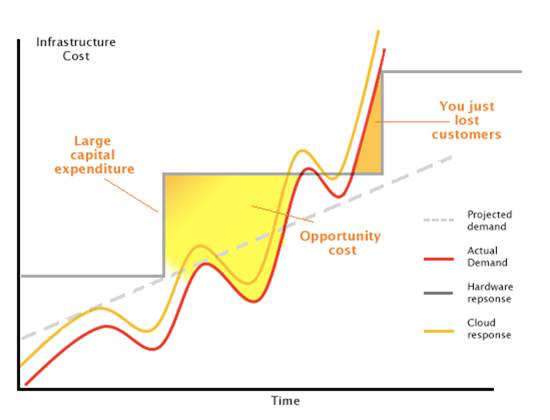
\includegraphics[scale=0.35]{images/elasticity.png}
			\end{figure}
			\begin{flushright}
				\tiny{source: \url{https://goo.gl/EzhyD5}}
			\end{flushright}
		\end{column}
	\end{columns}
\end{frame}

\subsection{Requirements}
\begin{frame}{Requirements}
	\only<1>
	{
		\begin{columns}
			\begin{column}{0.6\textwidth}
				elasticity major requirements
				\begin{itemize}
					\item{\footnotesize{from definition of elasticity}}
					\begin{itemize}
						\item{\scriptsize{autonomy}}
						\item{\scriptsize{scalability $\rightarrow{}$ \textbf{focus on horizontal}}}
						\item{\scriptsize{adaptability}}
					\end{itemize}
					\item{\footnotesize{specific for PaaS layer}}
					\begin{itemize}
						\item{\scriptsize{SLA-awareness}}
						\item{\scriptsize{composability}}
						\item{\scriptsize{service continuity in SW upgrades}}
					\end{itemize}
				\end{itemize}
			\end{column}
			\begin{column}{0.4\textwidth}
				\begin{figure}
					\centering{}
					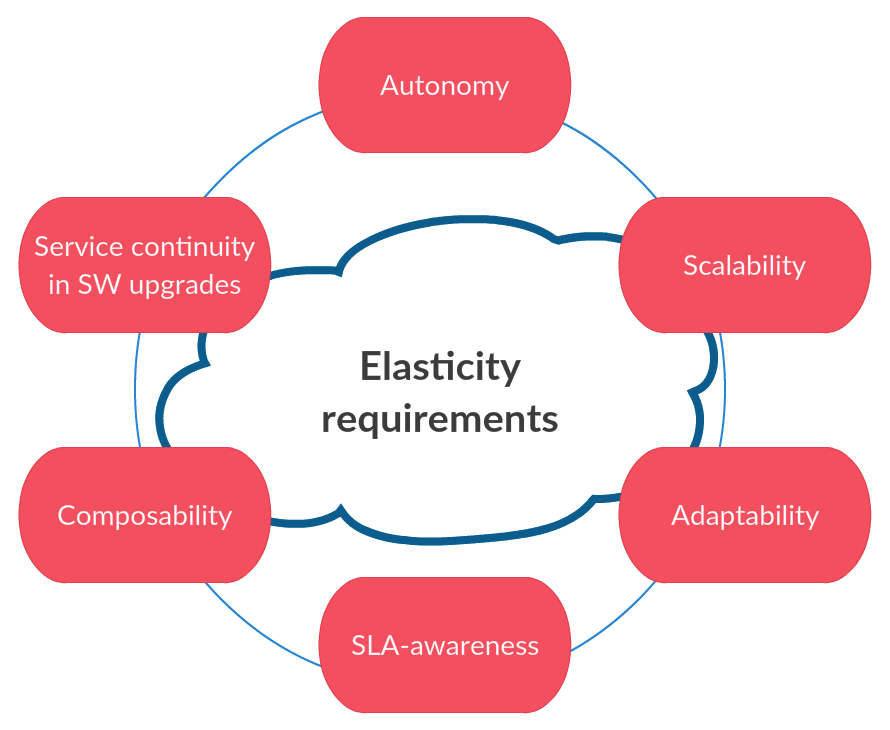
\includegraphics[scale=0.14]{images/elasticity-requirements.png}
				\end{figure}
			\end{column}
		\end{columns}
	}
	\only<2>
	{
		\begin{columns}
			\begin{column}{0.65\textwidth}
				scalability
				\begin{itemize}
					\item{\footnotesize{\textbf{replication (horizontal)}}}
					\begin{itemize}
						\item{\scriptsize{the only possible solution in PaaS}}
						\item{\scriptsize{PaaS manages units of deployments}}
					\end{itemize}
					\item{\footnotesize{some components are replicated when necessary}}
					\begin{itemize}
						\item{\scriptsize{the process must be transparent}}
						\item{\scriptsize{services must be well-designed}}
						\item{\scriptsize{classic architectures does not help}}
					\end{itemize}
					\item{\footnotesize{other}}
					\begin{itemize}
						\item{\scriptsize{redimension (vertical)}}
						\item{\scriptsize{migration}}
					\end{itemize}
				\end{itemize}
			\end{column}
			\begin{column}{0.35\textwidth}
				\begin{figure}
					\centering{}
					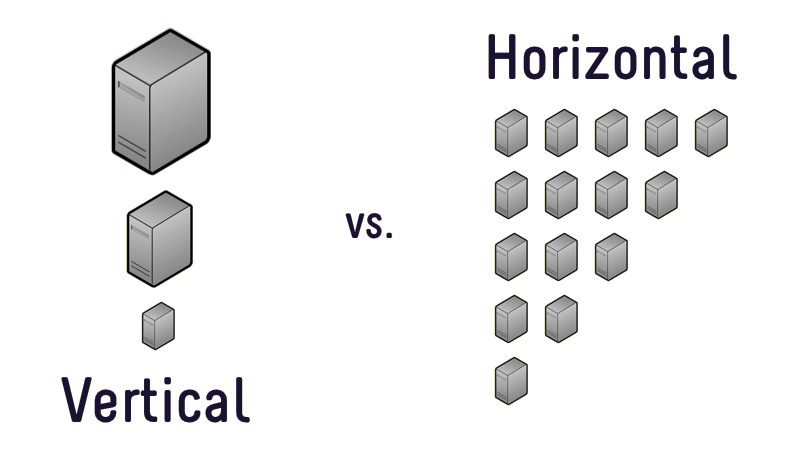
\includegraphics[scale=0.15]{images/scalability.png}
				\end{figure}
				\begin{flushright}
					\tiny{source: \url{https://goo.gl/orFWSi}}
				\end{flushright}
			\end{column}
		\end{columns}
	}
\end{frame}

\subsection{Multi-tenancy}
\begin{frame}{Multi-tenancy}
	\only<1>
	{
		\begin{columns}
			\begin{column}{0.57\textwidth}
				requirements
				\begin{itemize}
					\item{\footnotesize{availability $\rightarrow{}$ redundant services}}
					\item{\footnotesize{secure tenants isolation}}
					\item{\footnotesize{guarantee of service $\rightarrow$ performance}}
					\item{\footnotesize{management of underlying resources}}
				\end{itemize}
				\begin{center}
					providers have to plan SLA with a rich set of \textbf{objectives}
				\end{center}
			\end{column}
			\begin{column}{0.43\textwidth}
				\begin{figure}
					\centering{}
					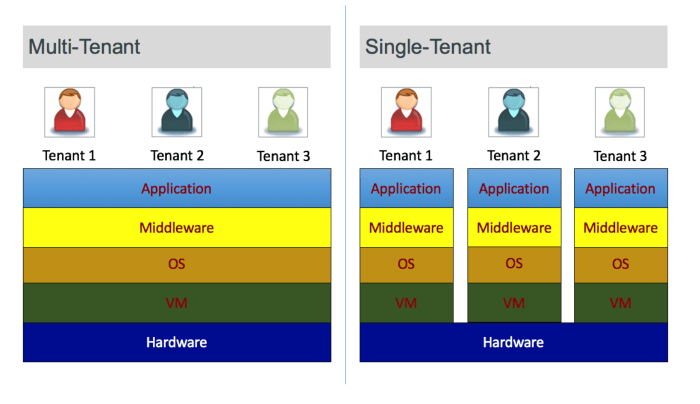
\includegraphics[scale=0.21]{images/multi-tenancy.png}
				\end{figure}
				\begin{flushright}
					\tiny{source: \url{http://goo.gl/MlsmWj}}
				\end{flushright}
			\end{column}
		\end{columns}
	}
	\only<2>
	{
		\begin{columns}
			\begin{column}{0.57\textwidth}
				naive architectures lead to
				\begin{itemize}
					\item{\footnotesize{inflexibility toward different needs}}
					\item{\footnotesize{security lacks}}
					\item{\footnotesize{inadequate usability}}
					\begin{itemize}
						\item{\scriptsize{sustain high workload $\rightarrow{}$ elasticity}}
					\end{itemize}
				\end{itemize}
			\end{column}
			\begin{column}{0.43\textwidth}
				\begin{figure}
					\centering{}
					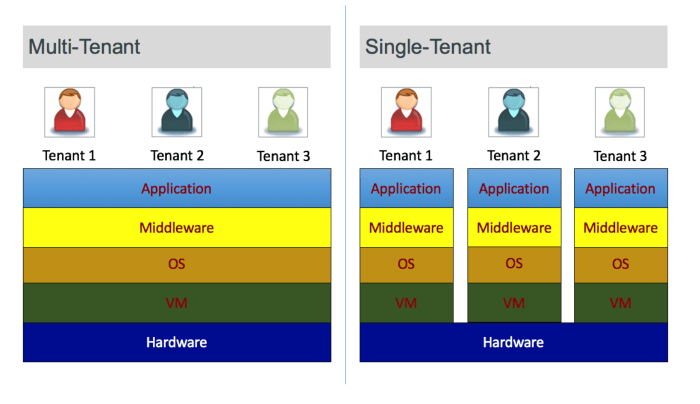
\includegraphics[scale=0.21]{images/multi-tenancy.png}
				\end{figure}
				\begin{flushright}
					\tiny{source: \url{http://goo.gl/MlsmWj}}
				\end{flushright}
			\end{column}
		\end{columns}
	}
\end{frame}
	%---------------------------------------------------------------------------------------------------
%		main.tex
%
%	This is the main file of the chapter that talk about elasticity and multi-tenancy.
%
%	Author: Andrea Meneghinello
% Version: 0.1
%	Table of changes:
%		12/03/2016 -> document definition
%---------------------------------------------------------------------------------------------------
\chapter{Elasticity}
\label{cap:solutionSpace}
%TODO -> chapter abstract

%--------------------------------------------------------------------------------------------------
% elasticity.tex
%
% This document define the frontespiece of the presentation
%
% author: Andrea Meneghinello
% version: 0.1
%--------------------------------------------------------------------------------------------------
\section{Elasticity}
\begin{frame}{Elasticity}
	\begin{columns}
		\begin{column}{0.5\textwidth}
			\textbf{elasticity} obtained by
			\begin{itemize}
				\item{\footnotesize{how PaaS exploits IaaS assets}}
				\begin{itemize}
					\item{\scriptsize{computing}}
					\item{\scriptsize{storage}}
					\item{\scriptsize{networking}}
				\end{itemize}
				\item{\footnotesize{how we build our services}}
				\begin{itemize}
					\item{\scriptsize{software architectures}}
					\item{\scriptsize{Software Engineering principles}}
				\end{itemize}
			\end{itemize}
		\end{column}
		\begin{column}{0.5\textwidth}
			\begin{figure}
				\centering{}
				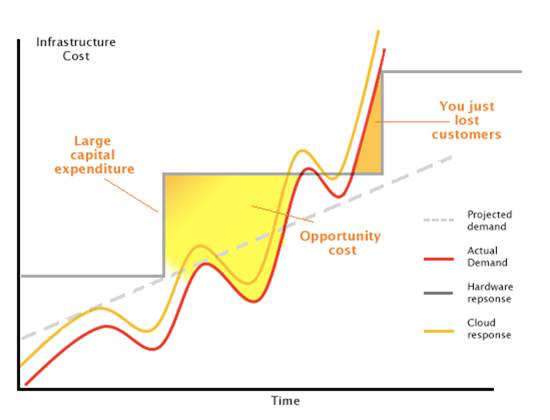
\includegraphics[scale=0.35]{images/elasticity.png}
			\end{figure}
			\begin{flushright}
				\tiny{source: \url{https://goo.gl/EzhyD5}}
			\end{flushright}
		\end{column}
	\end{columns}
\end{frame}

\subsection{Requirements}
\begin{frame}{Requirements}
	\only<1>
	{
		\begin{columns}
			\begin{column}{0.6\textwidth}
				elasticity major requirements
				\begin{itemize}
					\item{\footnotesize{from definition of elasticity}}
					\begin{itemize}
						\item{\scriptsize{autonomy}}
						\item{\scriptsize{scalability $\rightarrow{}$ \textbf{focus on horizontal}}}
						\item{\scriptsize{adaptability}}
					\end{itemize}
					\item{\footnotesize{specific for PaaS layer}}
					\begin{itemize}
						\item{\scriptsize{SLA-awareness}}
						\item{\scriptsize{composability}}
						\item{\scriptsize{service continuity in SW upgrades}}
					\end{itemize}
				\end{itemize}
			\end{column}
			\begin{column}{0.4\textwidth}
				\begin{figure}
					\centering{}
					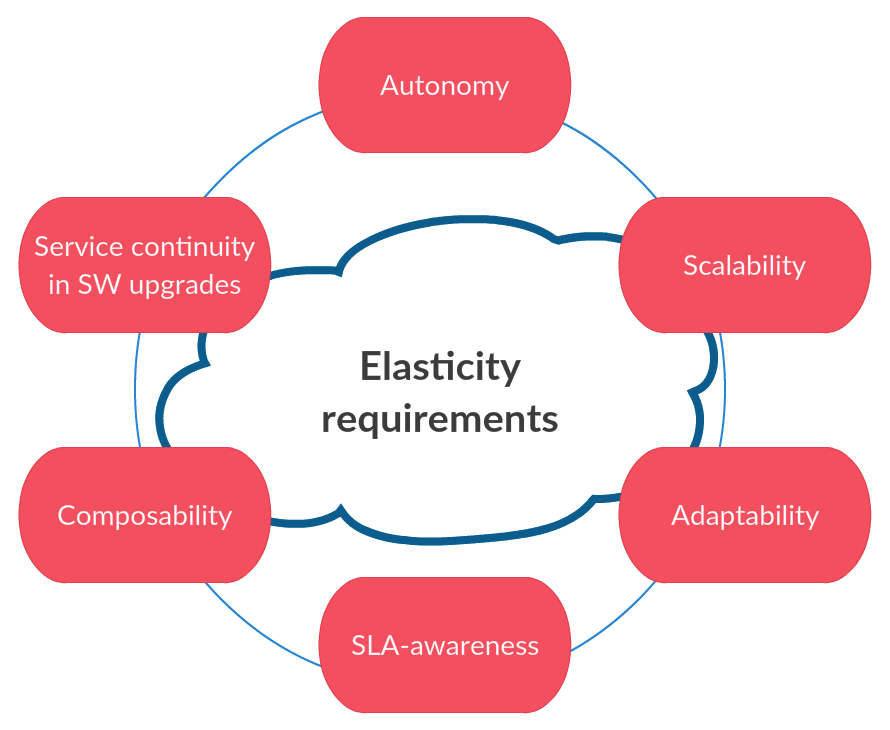
\includegraphics[scale=0.14]{images/elasticity-requirements.png}
				\end{figure}
			\end{column}
		\end{columns}
	}
	\only<2>
	{
		\begin{columns}
			\begin{column}{0.65\textwidth}
				scalability
				\begin{itemize}
					\item{\footnotesize{\textbf{replication (horizontal)}}}
					\begin{itemize}
						\item{\scriptsize{the only possible solution in PaaS}}
						\item{\scriptsize{PaaS manages units of deployments}}
					\end{itemize}
					\item{\footnotesize{some components are replicated when necessary}}
					\begin{itemize}
						\item{\scriptsize{the process must be transparent}}
						\item{\scriptsize{services must be well-designed}}
						\item{\scriptsize{classic architectures does not help}}
					\end{itemize}
					\item{\footnotesize{other}}
					\begin{itemize}
						\item{\scriptsize{redimension (vertical)}}
						\item{\scriptsize{migration}}
					\end{itemize}
				\end{itemize}
			\end{column}
			\begin{column}{0.35\textwidth}
				\begin{figure}
					\centering{}
					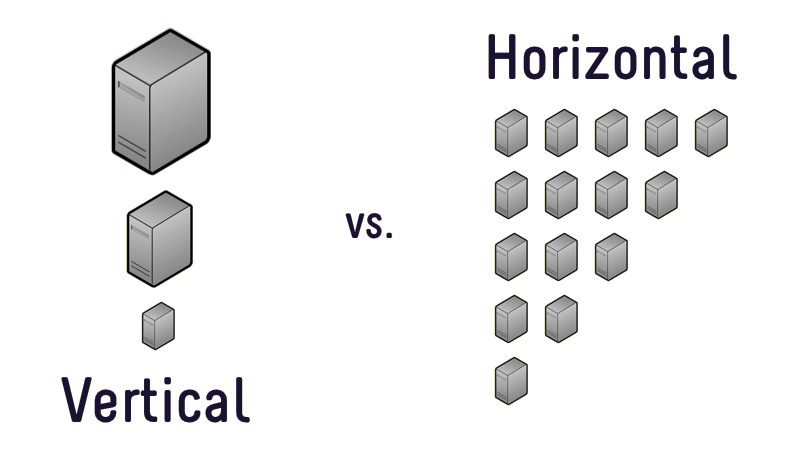
\includegraphics[scale=0.15]{images/scalability.png}
				\end{figure}
				\begin{flushright}
					\tiny{source: \url{https://goo.gl/orFWSi}}
				\end{flushright}
			\end{column}
		\end{columns}
	}
\end{frame}

\subsection{Multi-tenancy}
\begin{frame}{Multi-tenancy}
	\only<1>
	{
		\begin{columns}
			\begin{column}{0.57\textwidth}
				requirements
				\begin{itemize}
					\item{\footnotesize{availability $\rightarrow{}$ redundant services}}
					\item{\footnotesize{secure tenants isolation}}
					\item{\footnotesize{guarantee of service $\rightarrow$ performance}}
					\item{\footnotesize{management of underlying resources}}
				\end{itemize}
				\begin{center}
					providers have to plan SLA with a rich set of \textbf{objectives}
				\end{center}
			\end{column}
			\begin{column}{0.43\textwidth}
				\begin{figure}
					\centering{}
					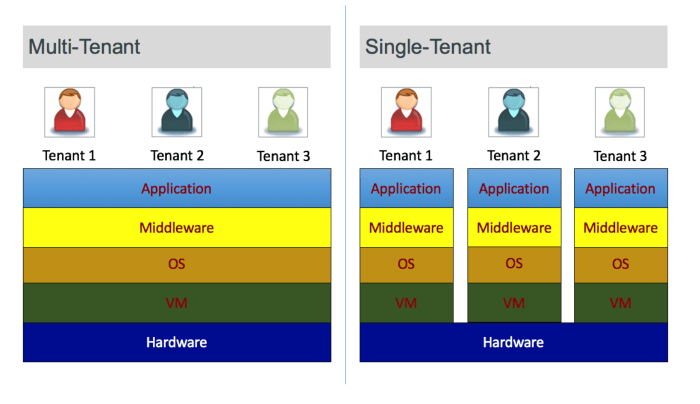
\includegraphics[scale=0.21]{images/multi-tenancy.png}
				\end{figure}
				\begin{flushright}
					\tiny{source: \url{http://goo.gl/MlsmWj}}
				\end{flushright}
			\end{column}
		\end{columns}
	}
	\only<2>
	{
		\begin{columns}
			\begin{column}{0.57\textwidth}
				naive architectures lead to
				\begin{itemize}
					\item{\footnotesize{inflexibility toward different needs}}
					\item{\footnotesize{security lacks}}
					\item{\footnotesize{inadequate usability}}
					\begin{itemize}
						\item{\scriptsize{sustain high workload $\rightarrow{}$ elasticity}}
					\end{itemize}
				\end{itemize}
			\end{column}
			\begin{column}{0.43\textwidth}
				\begin{figure}
					\centering{}
					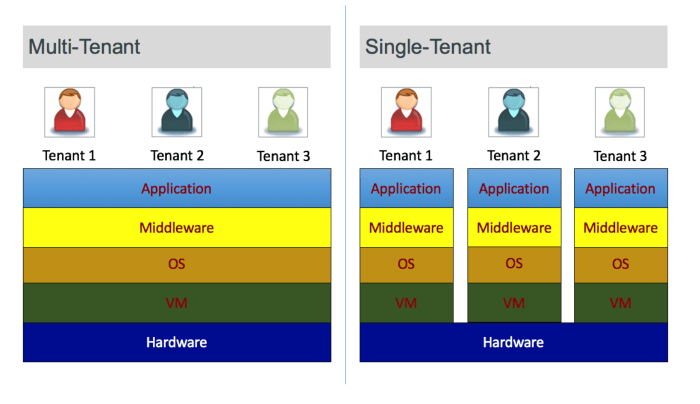
\includegraphics[scale=0.21]{images/multi-tenancy.png}
				\end{figure}
				\begin{flushright}
					\tiny{source: \url{http://goo.gl/MlsmWj}}
				\end{flushright}
			\end{column}
		\end{columns}
	}
\end{frame}
	%---------------------------------------------------------------------------------------------------
%		main.tex
%
%	This is the main file of the chapter that talk about elasticity and multi-tenancy.
%
%	Author: Andrea Meneghinello
% Version: 0.1
%	Table of changes:
%		12/03/2016 -> document definition
%---------------------------------------------------------------------------------------------------
\chapter{Elasticity}
\label{cap:solutionSpace}
%TODO -> chapter abstract

%--------------------------------------------------------------------------------------------------
% elasticity.tex
%
% This document define the frontespiece of the presentation
%
% author: Andrea Meneghinello
% version: 0.1
%--------------------------------------------------------------------------------------------------
\section{Elasticity}
\begin{frame}{Elasticity}
	\begin{columns}
		\begin{column}{0.5\textwidth}
			\textbf{elasticity} obtained by
			\begin{itemize}
				\item{\footnotesize{how PaaS exploits IaaS assets}}
				\begin{itemize}
					\item{\scriptsize{computing}}
					\item{\scriptsize{storage}}
					\item{\scriptsize{networking}}
				\end{itemize}
				\item{\footnotesize{how we build our services}}
				\begin{itemize}
					\item{\scriptsize{software architectures}}
					\item{\scriptsize{Software Engineering principles}}
				\end{itemize}
			\end{itemize}
		\end{column}
		\begin{column}{0.5\textwidth}
			\begin{figure}
				\centering{}
				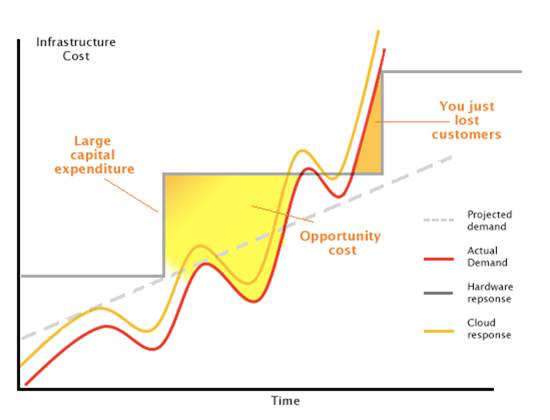
\includegraphics[scale=0.35]{images/elasticity.png}
			\end{figure}
			\begin{flushright}
				\tiny{source: \url{https://goo.gl/EzhyD5}}
			\end{flushright}
		\end{column}
	\end{columns}
\end{frame}

\subsection{Requirements}
\begin{frame}{Requirements}
	\only<1>
	{
		\begin{columns}
			\begin{column}{0.6\textwidth}
				elasticity major requirements
				\begin{itemize}
					\item{\footnotesize{from definition of elasticity}}
					\begin{itemize}
						\item{\scriptsize{autonomy}}
						\item{\scriptsize{scalability $\rightarrow{}$ \textbf{focus on horizontal}}}
						\item{\scriptsize{adaptability}}
					\end{itemize}
					\item{\footnotesize{specific for PaaS layer}}
					\begin{itemize}
						\item{\scriptsize{SLA-awareness}}
						\item{\scriptsize{composability}}
						\item{\scriptsize{service continuity in SW upgrades}}
					\end{itemize}
				\end{itemize}
			\end{column}
			\begin{column}{0.4\textwidth}
				\begin{figure}
					\centering{}
					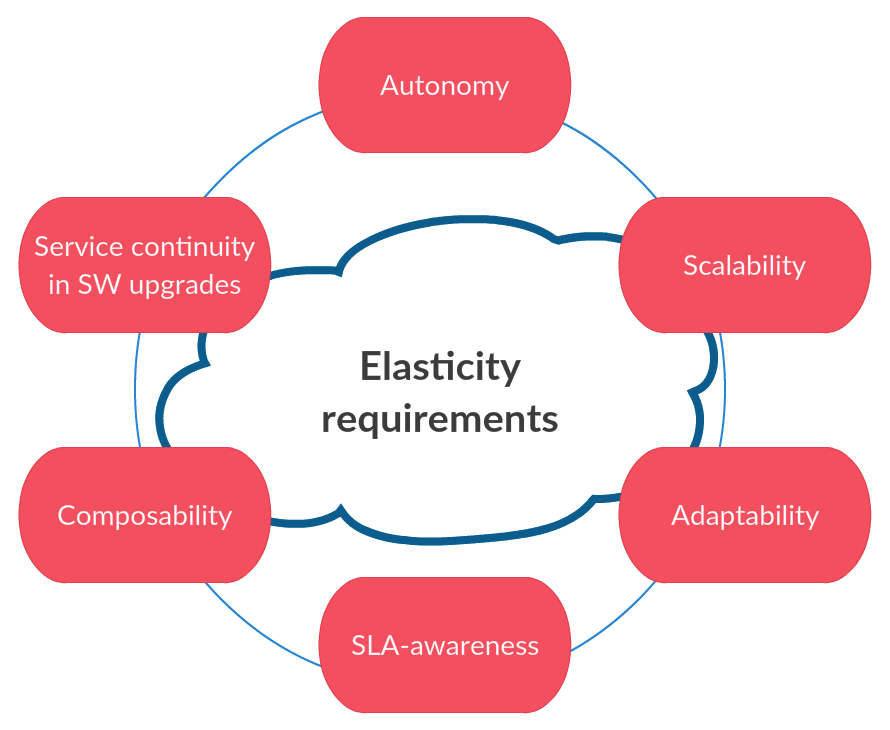
\includegraphics[scale=0.14]{images/elasticity-requirements.png}
				\end{figure}
			\end{column}
		\end{columns}
	}
	\only<2>
	{
		\begin{columns}
			\begin{column}{0.65\textwidth}
				scalability
				\begin{itemize}
					\item{\footnotesize{\textbf{replication (horizontal)}}}
					\begin{itemize}
						\item{\scriptsize{the only possible solution in PaaS}}
						\item{\scriptsize{PaaS manages units of deployments}}
					\end{itemize}
					\item{\footnotesize{some components are replicated when necessary}}
					\begin{itemize}
						\item{\scriptsize{the process must be transparent}}
						\item{\scriptsize{services must be well-designed}}
						\item{\scriptsize{classic architectures does not help}}
					\end{itemize}
					\item{\footnotesize{other}}
					\begin{itemize}
						\item{\scriptsize{redimension (vertical)}}
						\item{\scriptsize{migration}}
					\end{itemize}
				\end{itemize}
			\end{column}
			\begin{column}{0.35\textwidth}
				\begin{figure}
					\centering{}
					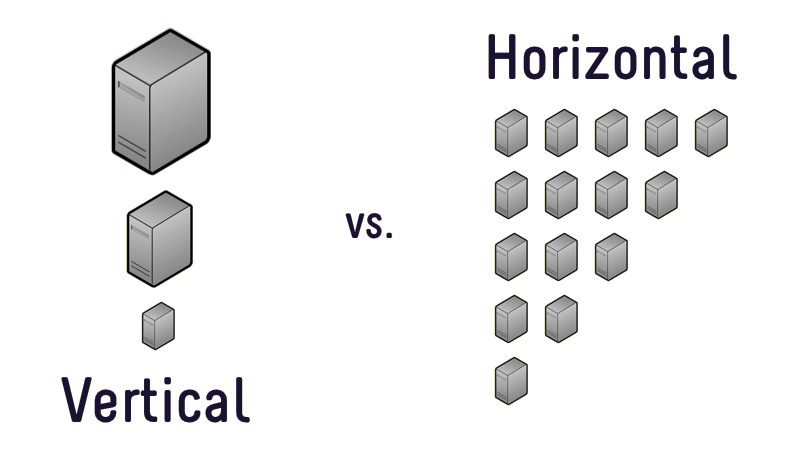
\includegraphics[scale=0.15]{images/scalability.png}
				\end{figure}
				\begin{flushright}
					\tiny{source: \url{https://goo.gl/orFWSi}}
				\end{flushright}
			\end{column}
		\end{columns}
	}
\end{frame}

\subsection{Multi-tenancy}
\begin{frame}{Multi-tenancy}
	\only<1>
	{
		\begin{columns}
			\begin{column}{0.57\textwidth}
				requirements
				\begin{itemize}
					\item{\footnotesize{availability $\rightarrow{}$ redundant services}}
					\item{\footnotesize{secure tenants isolation}}
					\item{\footnotesize{guarantee of service $\rightarrow$ performance}}
					\item{\footnotesize{management of underlying resources}}
				\end{itemize}
				\begin{center}
					providers have to plan SLA with a rich set of \textbf{objectives}
				\end{center}
			\end{column}
			\begin{column}{0.43\textwidth}
				\begin{figure}
					\centering{}
					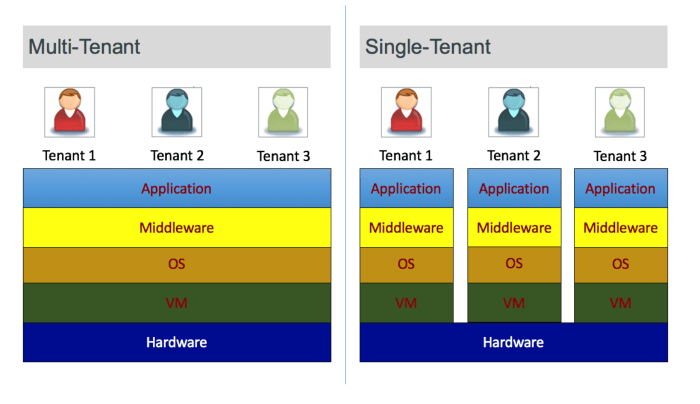
\includegraphics[scale=0.21]{images/multi-tenancy.png}
				\end{figure}
				\begin{flushright}
					\tiny{source: \url{http://goo.gl/MlsmWj}}
				\end{flushright}
			\end{column}
		\end{columns}
	}
	\only<2>
	{
		\begin{columns}
			\begin{column}{0.57\textwidth}
				naive architectures lead to
				\begin{itemize}
					\item{\footnotesize{inflexibility toward different needs}}
					\item{\footnotesize{security lacks}}
					\item{\footnotesize{inadequate usability}}
					\begin{itemize}
						\item{\scriptsize{sustain high workload $\rightarrow{}$ elasticity}}
					\end{itemize}
				\end{itemize}
			\end{column}
			\begin{column}{0.43\textwidth}
				\begin{figure}
					\centering{}
					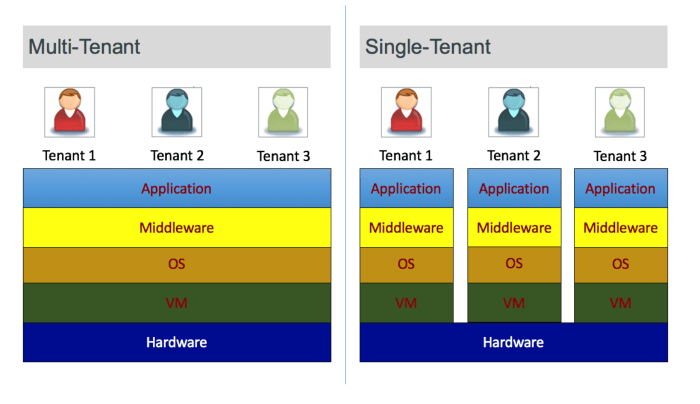
\includegraphics[scale=0.21]{images/multi-tenancy.png}
				\end{figure}
				\begin{flushright}
					\tiny{source: \url{http://goo.gl/MlsmWj}}
				\end{flushright}
			\end{column}
		\end{columns}
	}
\end{frame}
	
	%
	%	Glossary
	%
	\printGLS{\TRUE{}}
	
	%
	%	Appendices
	%
%	\begin{appendices}
%	\end{appendices}
	
	%
	%	Bibliography
	%
	\addcontentsline{toc}{chapter}{Biblography}
	\printbibliography[title=\textsc{Bibliography}]
\end{document}